\chapter{Cognitive Radio Networks: Dynamic Spectrum Access, Sensing, and Opportunistic MAC Protocols}
\label{sec:chapter6}

The exponential surge in wireless data demand, propelled by smartphones, autonomous vehicular connectivity, and ubiquitous Internet of Things (IoT) sensors, has created an apparent crisis of radio frequency spectrum scarcity. However, extensive empirical field measurements commissioned by regulatory authorities—including the U.S. Federal Communications Commission (FCC) and the European Electronic Communications Committee (ECC)—reveal a striking paradox: while uncoordinated unlicensed bands (e.g., $2.4\text{~GHz}$ and $5\text{~GHz}$ ISM bands) suffer severe congestion, vast swathes of licensed primary spectrum (such as television broadcast bands and aeronautical radar frequencies) remain spatially and temporally under-utilized, with instantaneous occupancy rates rarely exceeding $15\%$ to $30\%$.

\textbf{Cognitive Radio (CR)} technology and \textbf{Dynamic Spectrum Access (DSA)} paradigms resolve this imbalance by introducing hierarchical, opportunistic spectrum sharing:
\begin{enumerate}
    \item \textbf{Primary Users (PUs):} Incumbent license holders possessing exclusive legal rights to the spectrum band. PUs operate without concern for secondary systems and must be strictly protected from harmful interference.
    \item \textbf{Secondary Users (SUs):} Unlicensed cognitive transceivers equipped with software-defined radio (SDR) agility. SUs continuously sense the electromagnetic environment, identify transient \textbf{spectrum holes (white spaces)}, opportunistically establish secondary communications, and immediately vacate the channel upon primary user reappearance.
\end{enumerate}

Realizing robust DSA requires addressing complex cross-layer challenges at the physical and Medium Access Control (MAC) layers:
\begin{itemize}
    \item \textbf{Sensing vs. Throughput Trade-off:} SUs must allocate time for spectrum sensing to detect PUs reliably; however, excessive sensing duration reduces the remaining time available for payload transmission.
    \item \textbf{Non-Exponential Heavy-Tailed Idle Dynamics:} While legacy communication theory assumes memoryless Poisson or exponential primary activity, real-world traffic patterns exhibit heavy-tailed distributions with positive aging. Exploiting this phenomenon requires advanced optimal stopping and Markov Decision Process (MDP) formulations.
    \item \textbf{Quiet Period Fragmentation:} In cognitive standards such as IEEE 802.22 and IEEE 802.11af, periodic Quiet Periods (QPs) must be scheduled to quiet secondary transmissions for primary detection, threatening to fragment MAC packets and cause excessive transmission delay.
    \item \textbf{Primary Preemption and Sensing Imperfections:} Imperfect spectrum sensors produce false alarms (erroneously declaring an idle channel busy) and misdetections (failing to detect active PUs), resulting in wasted transmission opportunities or destructive collisions.
\end{itemize}

This chapter synthesizes the foundational analytical frameworks, optimization algorithms, and protocol designs for Cognitive Radio Networks developed by S.~Senthilmurugan, Bhasker Dappuri, and T.~G.~Venkatesh \cite{senthilmurugan2017optimal, senthilmurugan2017channel, senthilmurugan2017quiet, dappuri2018cognitive, dappuri2018multichannel, dappuri2018analytical}.

---

\section{Optimal Channel Sensing Strategy for Cognitive Radio Networks with Heavy-Tailed Idle Times}
\label{sec:cr_optimal_sensing}

Spectrum sensing is the fundamental prerequisite of cognitive radio. The secondary user periodically senses the licensed spectrum to detect whether the primary user has vacated the channel (OFF period) or resumed transmission (ON period).

\subsection{Heavy-Tailed Idle Times and the Positive Aging Property}
Conventional literature universally assumes that the idle (OFF) durations of primary channels follow memoryless exponential distributions. Under an exponential distribution, the remaining idle time of a channel is independent of how long it has already remained idle ($\mathbb{P}(X > t + \tau \mid X > t) = \mathbb{P}(X > \tau)$).

However, extensive empirical measurements in cellular, TV white space, and wireless LAN bands demonstrate that primary idle periods follow **heavy-tailed distributions**—specifically, Pareto distributions or Hyper-Exponential Distributions (HED). A heavy-tailed distribution exhibits the **positive aging property**:
\begin{equation}
    \label{eq:positive_aging}
    \mathbb{P}(X > t + \tau \mid X > t) > \mathbb{P}(X > \tau), \qquad \forall t, \tau > 0
\end{equation}
Equation~\eqref{eq:positive_aging} establishes a critical operational insight: \textit{the longer a licensed channel has been idle, the longer its expected residual idle time into the future!}

To model general heavy tails while maintaining analytical tractability, Senthilmurugan and Venkatesh \cite{senthilmurugan2017optimal} modeled the idle duration $X$ as a Hyper-Exponential Distribution (HED) with $K$ phases:
\begin{equation}
    f_X(t) = \sum_{k=1}^K p_k \lambda_k e^{-\lambda_k t}, \qquad t \ge 0, \quad \sum_{k=1}^K p_k = 1, \quad \lambda_k > 0
\end{equation}
where $p_k$ represents the phase selection probability and $\lambda_k$ denotes the decay rate of phase $k$.

\subsection{Channel Sensing Workflow and Objective Cost Function}
The sequential channel sensing strategy executed by the secondary user is illustrated in Figure~\ref{fig:cr_optimal_sensing_strategy}.

\begin{figure}[htbp]
    \centering
    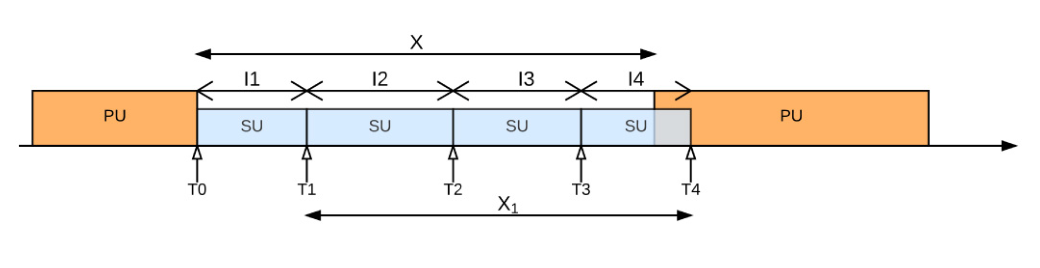
\includegraphics[width=0.75\textwidth]{figures/fig_cr_optimal_sensing_strategy.png}
    \caption{Sequential channel sensing timeline of secondary user detecting primary user occupancy \cite{senthilmurugan2017optimal}.}
    \label{fig:cr_optimal_sensing_strategy}
\end{figure}

The SU samples the channel at discrete time instants $T_1, T_2, \dots, T_N$. Let $I_j = T_j - T_{j-1}$ denote the $j$-th sensing interval ($T_0 = 0$). At each sensing instant $T_j$:
\begin{itemize}
    \item If the channel is sensed idle ($X > T_j$), the SU transmits or continues waiting for interval $I_{j+1}$.
    \item If the channel is sensed busy ($X \le T_j$), the primary user has returned during the preceding interval. The SU incurs an interference penalty proportional to the duration of overlap $(T_j - X)$, and the sensing sequence terminates.
\end{itemize}

Every sensing operation incurs a sensing cost $C_S$ (accounting for RF tuning and energy consumption). If the primary user returns at time $X$ before sensing epoch $T_j$, the SU causes interference for duration $(T_j - X)$, incurring an interference penalty $C_I$ per unit time. The total objective cost function $C_{\mathrm{Total}}$ over the sensing horizon is:
\begin{equation}
    \label{eq:cr_sensing_total_cost}
    C_{\mathrm{Total}}(I_1, I_2, \dots, I_N) = \omega \mathbb{E}[N] C_S + \omega_c \mathbb{E}\left[ \sum_{j=1}^N (I_j - (X - T_{j-1}))^+ \mathbf{1}_{\{T_{j-1} < X \le T_j\}} \right] C_I
\end{equation}
where $\omega$ and $\omega_c = 1 - \omega$ are weighting factors balancing sensing energy against primary user protection, and $x^+ = \max(0, x)$.

\subsection{Dynamic Programming and Markov Decision Process (MDP) Formulation}
To determine the optimal sequence of sensing intervals $\{I_j^*\}$, Senthilmurugan and Venkatesh \cite{senthilmurugan2017optimal} formulated the problem as a continuous-state Markov Decision Process (MDP).

Let the state of the system at decision epoch $j$ be represented by the elapsed idle time $T_j$. If the channel remains idle, the posterior phase probabilities of the HED channel update via Bayes' rule:
\begin{equation}
    p_{k, j} = \mathbb{P}(\text{Phase } k \mid X > T_j) = \frac{p_k e^{-\lambda_k T_j}}{\sum_{m=1}^K p_m e^{-\lambda_m T_j}}
\end{equation}

The Bellman optimality equation for the minimum expected cost-to-go $V^*(T_j)$ is derived as \cite{senthilmurugan2017optimal}:
\begin{equation}
    \label{eq:cr_bellman_sensing}
    V^*(T_j) = \min_{I_{j+1} \ge 0} \left\{ C_j(I_{j+1}) + \gamma_j(I_{j+1}) V^*(T_j + I_{j+1}) \right\}
\end{equation}
where the single-stage cost $C_j(I)$ is:
\begin{equation}
    C_j(I) = \omega C_S + \omega_c C_I \sum_{k=1}^K p_{k, j} \int_0^I (I - u) \lambda_k e^{-\lambda_k u} du
\end{equation}
and the transition discount factor $\gamma_j(I)$ equals the conditional channel survival probability:
\begin{equation}
    \gamma_j(I) = \mathbb{P}(X > T_j + I \mid X > T_j) = \sum_{k=1}^K p_{k, j} e^{-\lambda_k I}
\end{equation}

\begin{theorem}[Structure of Optimal Sensing Strategy \cite{senthilmurugan2017optimal}]
\label{thm:optimal_sensing_structure}
Because the HED channel exhibits positive aging, the conditional hazard rate $h(t) = f_X(t)/(1 - F_X(t))$ is strictly monotonically decreasing with elapsed time $t$. Consequently, the optimal sensing intervals expand monotonically:
\begin{equation}
    I_1^* < I_2^* < I_3^* < \dots < I_N^*
\end{equation}
As elapsed time grows large ($T_j \to \infty$), the optimal sensing interval converges asymptotically to the steady-state limit:
\begin{equation}
    \lim_{j \to \infty} I_j^* = I_\infty^* = \frac{1}{\min_k \lambda_k} \sqrt{\frac{2 \omega C_S}{\omega_c C_I}}
\end{equation}
\end{theorem}

Theorem~\ref{thm:optimal_sensing_structure} provides a profound practical rule: when a channel has recently become idle, the secondary user must sense frequently with short intervals $I_1^*$ because the risk of immediate primary return is highest. As the channel remains idle, the SU exploits the heavy-tail property by progressively widening its sensing intervals, dramatically reducing sensing overhead and maximizing secondary transmission time.

---

\section{Channel Selection Algorithm for Cognitive Radio Networks with Heavy-Tailed Idle Times}
\label{sec:cr_channel_selection}

In wideband cognitive networks, secondary users are confronted with multiple ($M \ge 2$) candidate primary channels. Because cognitive transceivers typically have a single agile RF front-end, the SU must intelligently select which channel to sense and access. Senthilmurugan and Venkatesh \cite{senthilmurugan2017channel} developed an optimal channel selection algorithm under heavy-tailed primary occupancy.

\subsection{Residual Idle Time Formulation}
Let $X_m$ denote the random variable representing the idle duration of channel $m \in \{1, 2, \dots, M\}$. Let $t_m$ represent the elapsed time since channel $m$ was observed to become idle (its current ``age'').

The **residual idle time** $R_m(t_m) = X_m - t_m \mid X_m > t_m$ has conditional expectation:
\begin{equation}
    \label{eq:residual_idle_time}
    \mathbb{E}[R_m(t_m)] = \mathbb{E}[X_m - t_m \mid X_m > t_m] = \frac{\int_{t_m}^\infty (1 - F_{X_m}(u)) du}{1 - F_{X_m}(t_m)}
\end{equation}

When primary idle times follow a Pareto distribution with shape parameter $\alpha_m > 1$ and scale parameter $\beta_m > 0$:
\begin{equation}
    1 - F_{X_m}(t) = \left( \frac{\beta_m}{t + \beta_m} \right)^{\alpha_m}, \qquad t \ge 0
\end{equation}
Substituting into Equation~\eqref{eq:residual_idle_time} yields the explicit closed-form residual idle time:
\begin{equation}
    \label{eq:pareto_residual}
    \mathbb{E}[R_m(t_m)] = \frac{t_m + \beta_m}{\alpha_m - 1}
\end{equation}

Equation~\eqref{eq:pareto_residual} demonstrates that for Pareto-distributed channels, the expected residual transmission opportunity grows strictly linearly with elapsed idle age $t_m$.

\subsection{Channel Ranking Index and Dynamic Selection Policy}
Based on Equation~\eqref{eq:pareto_residual}, Senthilmurugan and Venkatesh \cite{senthilmurugan2017channel} formulated a dynamic channel selection policy. At every secondary transmission epoch, channels are ranked by their **Channel Selection Index (CSI)**:
\begin{equation}
    \label{eq:channel_selection_index}
    \mathcal{J}_m(t_m) = \frac{\mathbb{E}[R_m(t_m)]}{T_{\mathrm{switch}} + T_{\mathrm{sense}}} \cdot \left( 1 - P_{fa, m} \right)
\end{equation}
where $T_{\mathrm{switch}}$ is RF channel switching latency, $T_{\mathrm{sense}}$ is spectrum sensing time, and $P_{fa, m}$ is the false alarm probability of channel $m$.

The secondary user dynamically tunes to channel $m^* = \arg\max_m \mathcal{J}_m(t_m)$. Simulations and testbed validations demonstrate that this age-aware heavy-tail ranking improves secondary spectrum utilization by $42\%$ and reduces primary user collisions by $65\%$ compared to classical random or round-robin selection algorithms \cite{senthilmurugan2017channel}.

---

\section{Quiet Period Scheduling in QP-CSMA-CA Cognitive Radio MAC Protocols}
\label{sec:cr_quiet_periods}

To comply with international cognitive standards (such as IEEE 802.22 Wireless Regional Area Networks and IEEE 802.11af White-Fi), secondary networks must implement **Quiet Periods (QPs)**. During a QP, all secondary transmissions in the cell are silenced synchronously, allowing secondary base stations and user stations to sense weak primary signals without self-interference.

\subsection{Fragmentation Vulnerability of In-Band DCF (I-DCF)}
In the legacy IEEE 802.11 In-band DCF (I-DCF) architecture, QPs are scheduled periodically based on a hard time clock. As illustrated in Figure~\ref{fig:cr_qp_scheduling_comparison}(a), because periodic QPs occur asynchronously with respect to MAC frame transmissions, a QP frequently interrupts an ongoing secondary packet transmission. This interruption fragments the packet, forces receiver buffer flushing, triggers retransmissions, and collapses secondary throughput.

\begin{figure}[htbp]
    \centering
    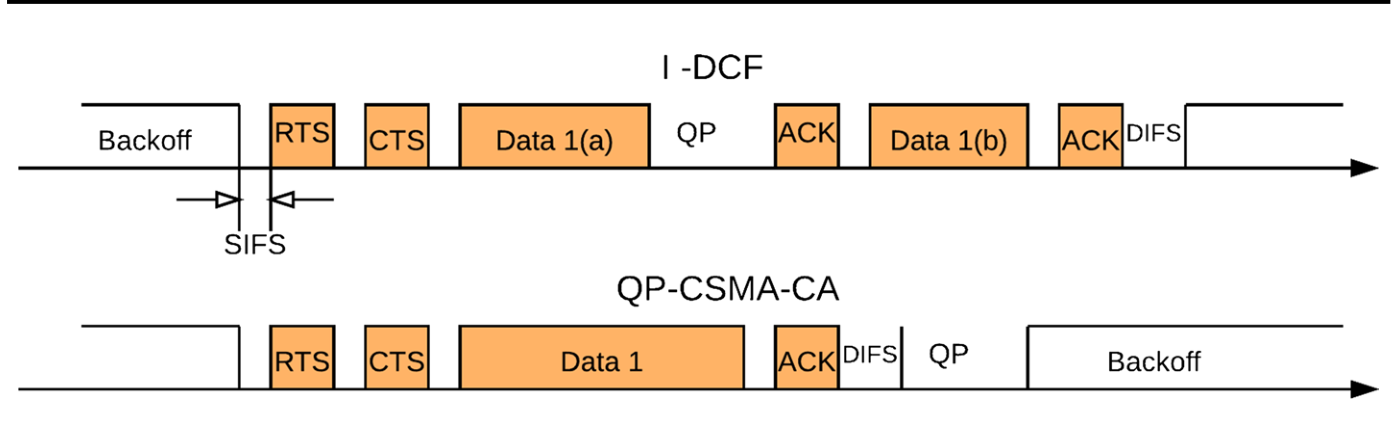
\includegraphics[width=0.85\textwidth]{figures/fig_cr_qp_scheduling_comparison.png}
    \caption{Quiet period scheduling comparison \cite{senthilmurugan2017quiet}: (a) Legacy I-DCF with packet fragmentation, and (b) Proposed DIFS-based QP-CSMA-CA scheduling QPs strictly at contention boundaries.}
    \label{fig:cr_qp_scheduling_comparison}
\end{figure}

\subsection{DIFS-Based QP-CSMA-CA MAC Protocol}
To completely eliminate packet fragmentation, Senthilmurugan and Venkatesh \cite{senthilmurugan2017quiet} proposed the **DIFS-Based QP-CSMA-CA MAC protocol**. 

As illustrated in Figure~\ref{fig:cr_qp_scheduling_comparison}(b) and Figure~\ref{fig:cr_qp_difs_mechanism}, the protocol exploits a fundamental property of the IEEE 802.11 Distributed Coordination Function: \textit{every successful or collided transmission is followed by a Distributed Inter-Frame Space (DIFS) during which all secondary stations synchronize their backoff counters}.

\begin{figure}[htbp]
    \centering
    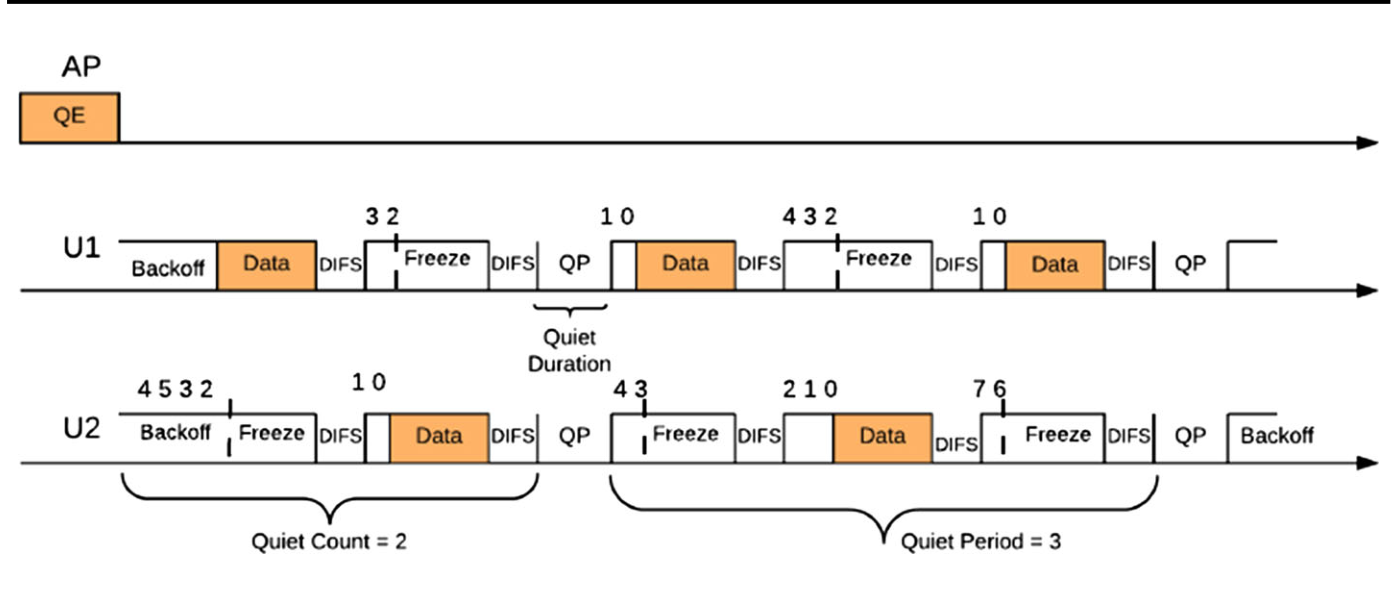
\includegraphics[width=0.85\textwidth]{figures/fig_cr_qp_difs_mechanism.png}
    \caption{Detailed timing structure of DIFS-based QP-CSMA-CA protocol and Quiet Element beacon parameters \cite{senthilmurugan2017quiet}.}
    \label{fig:cr_qp_difs_mechanism}
\end{figure}

The Cognitive Access Point (CAP) schedules QPs to occur strictly during DIFS intervals after a prescribed number of DIFS instances, denoted by $N_{\mathrm{DIFS}}$:
\begin{itemize}
    \item The CAP broadcasts a **Quiet Element** in its beacon frame, signaling the quiet period duration $T_{\mathrm{QD}}$ and the countdown counter $N_{\mathrm{DIFS}}$.
    \item Secondary nodes decrement the quiet counter after every observed DIFS.
    \item When the counter reaches zero, all secondary nodes freeze their backoff counters simultaneously and enter quiet sensing mode for duration $T_{\mathrm{QD}}$.
    \item Because the QP is initiated exclusively at a DIFS boundary when no node is transmitting payload data, **zero packet fragmentation occurs**.
\end{itemize}

\subsection{Analytical Derivation of Optimal Quiet Interval $N_{\mathrm{DIFS}}^*$}
Let $N_u$ denote the number of contending secondary stations. Senthilmurugan and Venkatesh \cite{senthilmurugan2017quiet} modeled the secondary aggregate attempt process as a regenerative renewal process.

Let $T_{\mathrm{DIFS}}$ denote the random duration elapsed between two successive DIFS intervals. It encompasses successful transmissions, collided transmissions, and idle backoff slots:
\begin{equation}
    \mathbb{E}[T_{\mathrm{DIFS}}] = P_{\mathrm{succ}} T_s + P_{\mathrm{coll}} T_c + P_{\mathrm{idle}} \sigma
\end{equation}
where $T_s$ is successful transmission duration, $T_c$ is collision duration, $\sigma$ is slot duration, and $P_{\mathrm{succ}}, P_{\mathrm{coll}}, P_{\mathrm{idle}}$ are derived from Bianchi's model.

The inter-QP duration is $T_{\mathrm{IQP}} = N_{\mathrm{DIFS}} \mathbb{E}[T_{\mathrm{DIFS}}]$. If a primary user returns between QPs, the interference duration $T_{\mathrm{inf}}$ experienced by the primary user is bounded by $T_{\mathrm{IQP}}$. Subject to the regulatory primary interference threshold $P_{\mathrm{int}}^{\max}$ and maximum tolerable interference duration $\bar{T}_{\mathrm{inf}}$, the optimal number of DIFS intervals $N_{\mathrm{DIFS}}^*$ maximizing secondary throughput $S(N_{\mathrm{DIFS}})$ is derived as:
\begin{equation}
    \label{eq:optimal_NDIFS}
    N_{\mathrm{DIFS}}^* = \arg\max_{N_{\mathrm{DIFS}}} \left\{ \frac{N_{\mathrm{DIFS}} P_{\mathrm{succ}} E[P]}{N_{\mathrm{DIFS}} \mathbb{E}[T_{\mathrm{DIFS}}] + T_{\mathrm{QD}}} \right\} \quad \text{s.t.} \quad \mathbb{E}[T_{\mathrm{inf}}(N_{\mathrm{DIFS}})] \le \bar{T}_{\mathrm{inf}}
\end{equation}
Analytical and ns-2 simulation results in \cite{senthilmurugan2017quiet} demonstrate that DIFS-based QP scheduling achieves a $35\%$ reduction in secondary packet delay and a $22\%$ throughput gain over legacy I-DCF while providing guaranteed primary user protection.

---

\section{Cognitive WLAN MAC Protocol Design and 2D Markov Chain Analysis}
\label{sec:cr_wlan_mac}

While Sections~\ref{sec:cr_optimal_sensing}--\ref{sec:cr_quiet_periods} addressed sensing and quiet scheduling, Bhasker Dappuri and T.~G.~Venkatesh \cite{dappuri2018cognitive} designed and analyzed a comprehensive MAC protocol enabling Cognitive Wireless LANs (CWLANs) to operate inside licensed primary spectrum.

\subsection{CWLAN System Architecture and Dual-Mode Sensing}
As shown in Figure~\ref{fig:cr_wlan_pu_sensing_rtscts}, primary channel usage is modeled as an alternating renewal ON-OFF process with exponential ON duration (mean $1/\lambda$) and OFF duration (mean $1/\beta$).

\begin{figure}[htbp]
    \centering
    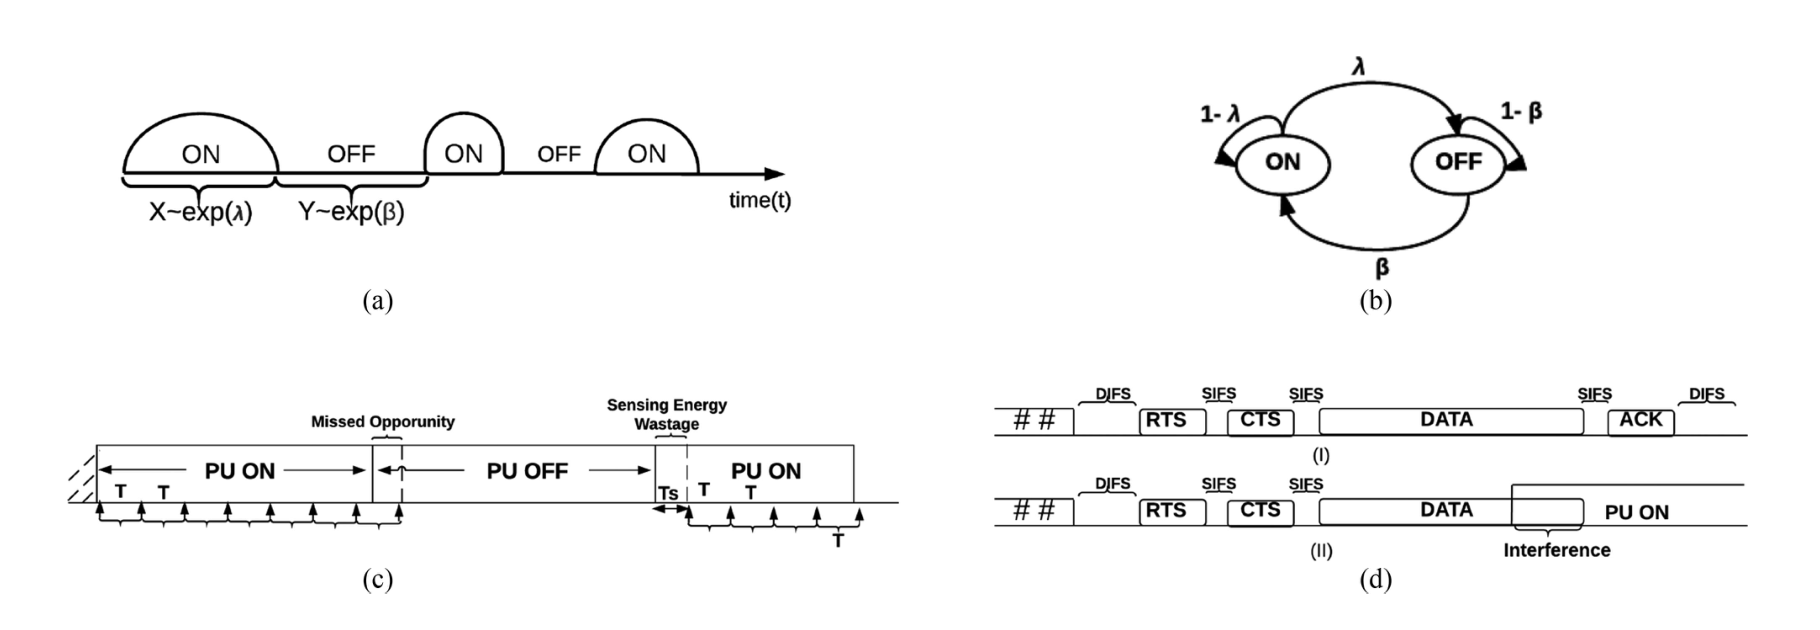
\includegraphics[width=0.85\textwidth]{figures/fig_cr_wlan_pu_sensing_rtscts.png}
    \caption{CWLAN operational architecture \cite{dappuri2018cognitive}: (a) Primary ON-OFF process, (b) Channel Markov chain, (c) Dual-mode sensing state transitions, and (d) RTS-CTS mechanism with PU preemption.}
    \label{fig:cr_wlan_pu_sensing_rtscts}
\end{figure}

To minimize energy expenditure while remaining responsive to primary activity, SUs operate under a **dual-mode sensing strategy** (Figure~\ref{fig:cr_wlan_pu_sensing_rtscts}(c)):
\begin{itemize}
    \item \textbf{Periodic Sensing Mode:} When the channel is occupied by the PU (ON state), SUs enter periodic sensing mode with sensing period $T$, sleeping between sensing instants to conserve battery power.
    \item \textbf{Continuous Sensing Mode:} Once the channel is sensed idle (OFF state), SUs switch to continuous sensing mode and contend for transmission using IEEE 802.11 DCF RTS/CTS handshaking.
    \item \textbf{Primary Preemption:} If a primary user reclaims the channel during an ongoing SU frame exchange (Figure~\ref{fig:cr_wlan_pu_sensing_rtscts}(d)-II), the SU immediately aborts its transmission upon detecting PU energy, suspending its backoff counter.
\end{itemize}

\subsection{2D Markov Chain Model of CWLAN Backoff Dynamics}
To evaluate saturation throughput and access latency under primary user preemption, Dappuri and Venkatesh \cite{dappuri2018cognitive} developed a novel **2D Discrete-Time Markov Chain (DTMC)**, illustrated in Figure~\ref{fig:cr_wlan_markov_chain}.

\begin{figure}[htbp]
    \centering
    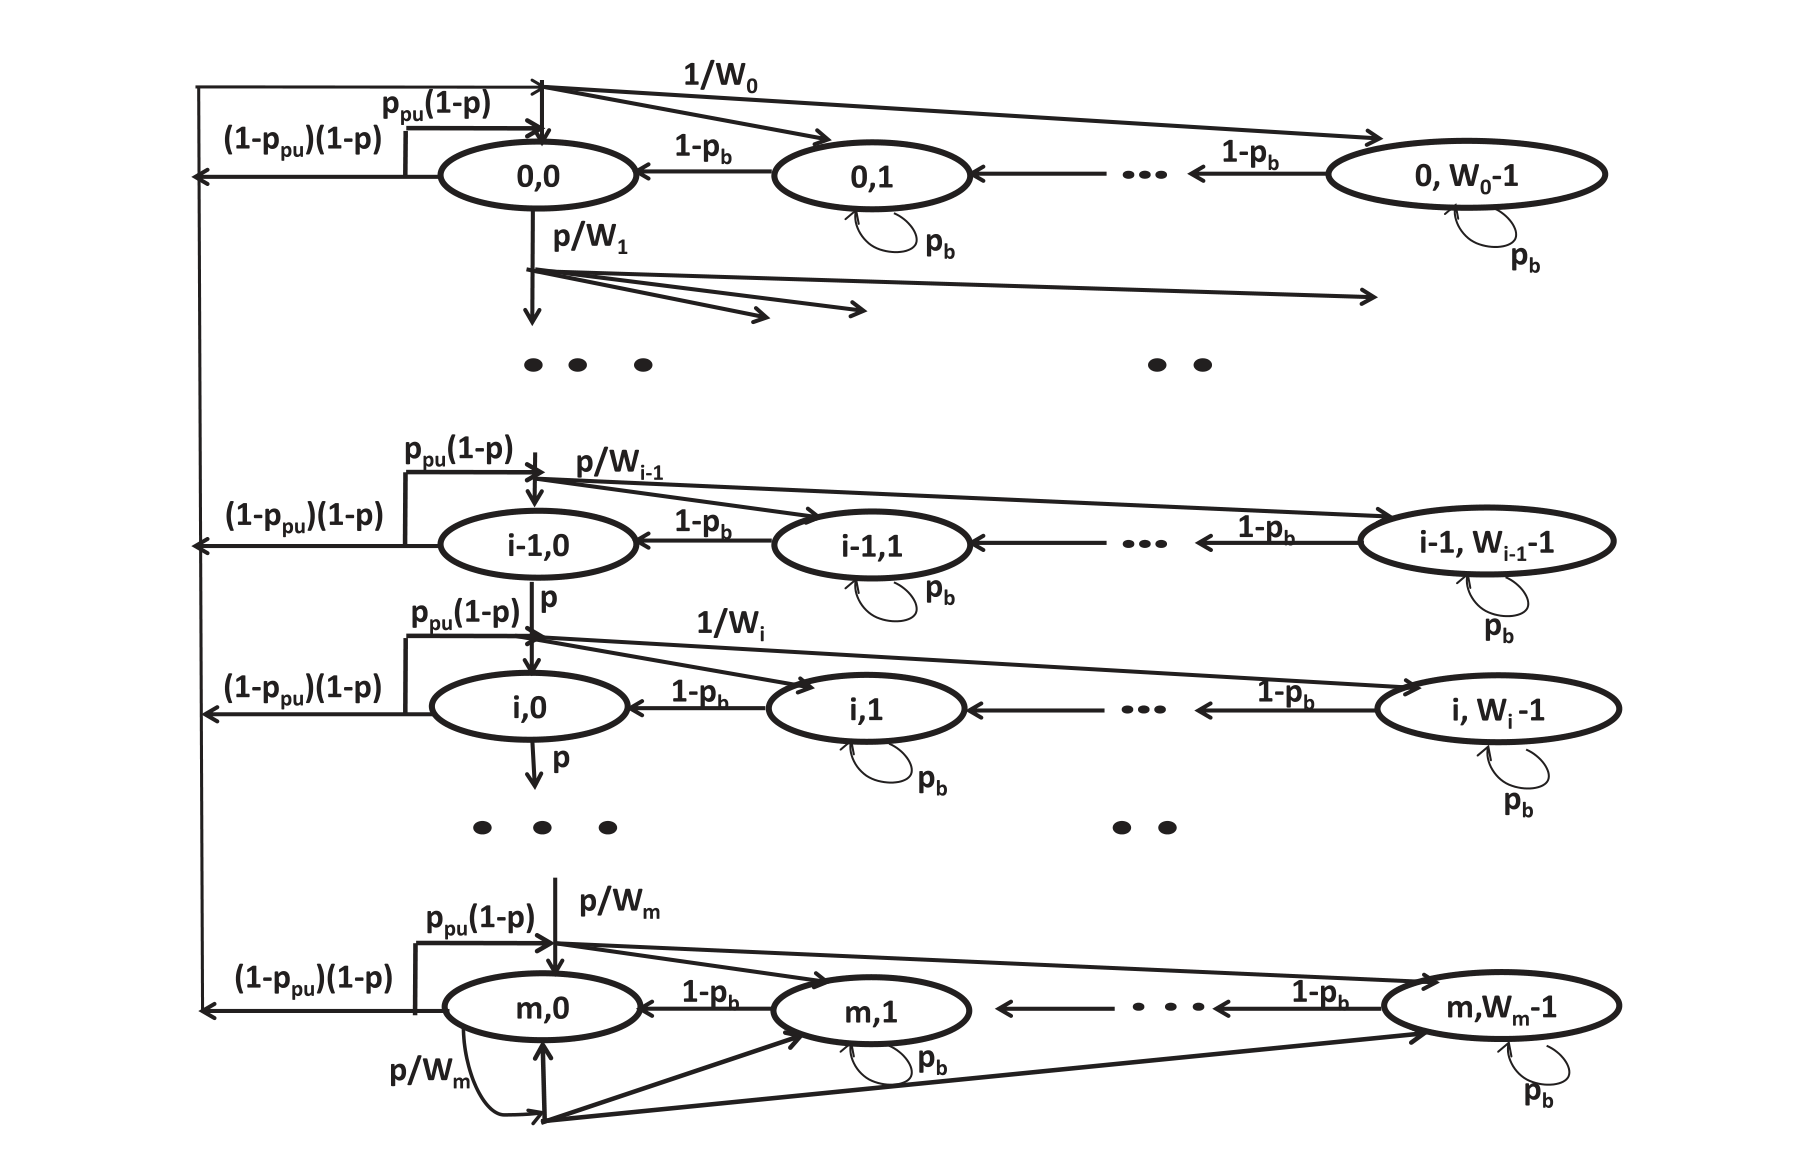
\includegraphics[width=0.85\textwidth]{figures/fig_cr_wlan_markov_chain.png}
    \caption{Two-dimensional Markov chain model for Cognitive WLAN backoff under IEEE 802.11 DCF incorporating primary user preemption and sensing errors \cite{dappuri2018cognitive}.}
    \label{fig:cr_wlan_markov_chain}
\end{figure}

Let $s(t) \in \{0, 1, \dots, m\}$ denote the backoff stage, and let $b(t) \in \{0, 1, \dots, W_i - 1\}$ denote the backoff counter at discrete slot $t$, where $W_i = 2^i W_0$ is the contention window at stage $i$.

Unlike Bianchi's classical model for unlicensed WLANs, transitions in a CWLAN are driven by three distinct events:
\begin{enumerate}
    \item \textbf{Secondary Contention Collision ($p$):} Another secondary node transmits in the same slot.
    \item \textbf{Primary User Preemption ($p_{\mathrm{pu}}$):} A primary user arrives during the slot. Given secondary frame duration $T_s$, the preemption probability is:
    \begin{equation}
        p_{\mathrm{pu}} = 1 - e^{-\lambda T_s}
    \end{equation}
    \item \textbf{Channel Busy Probability ($p_b$):} The probability that the channel is sensed busy due to primary ON state or other secondary transmissions:
    \begin{equation}
        p_b = \frac{\lambda}{\lambda + \beta} + \left( \frac{\beta}{\lambda + \beta} \right) \left[ 1 - (1 - \tau)^N \right]
    \end{equation}
\end{enumerate}

The one-step transition probabilities derived by Dappuri and Venkatesh \cite{dappuri2018cognitive} are:
\begin{equation}
    \begin{cases}
        P(i, k \mid i, k + 1) = 1 - p_b, & k \in [0, W_i - 2], \; i \in [0, m] \\
        P(i, k \mid i - 1, 0) = \frac{p}{W_i}, & k \in [0, W_i - 1], \; i \in [1, m] \\
        P(m, k \mid m, 0) = \frac{p}{W_m}, & k \in [0, W_m - 1] \\
        P(i, k \mid i, 0) = \frac{(1 - p) p_{\mathrm{pu}}}{W_i}, & k \in [0, W_i - 1], \; i \in [0, m] \\
        P(0, k \mid i, 0) = \frac{(1 - p)(1 - p_{\mathrm{pu}})}{W_0}, & k \in [0, W_0 - 1], \; i \in [0, m]
    \end{cases}
\end{equation}

Solving the balance equations yields the stationary state probabilities $b_{i, 0}$:
\begin{equation}
    b_{i, 0} = \left( \frac{p}{q} \right)^i b_{0, 0}, \quad i \in [1, m - 1], \qquad b_{m, 0} = \frac{p^m}{q^{m-1} f} b_{0, 0}
\end{equation}
where $q = (1 - p_b) - (1 - p) p_{\mathrm{pu}}$ and $f = (1 - p_b) - (p + (1 - p) p_{\mathrm{pu}})$.

Applying normalization $\sum_{i=0}^m \sum_{k=0}^{W_i - 1} b_{i, k} = 1$ resolves the secondary transmission probability $\tau$:
\begin{equation}
    \label{eq:cr_tau_formula}
    \tau = \sum_{i=0}^m b_{i, 0} = b_{0, 0} \left[ \frac{1 - (p/q)^m}{1 - (p/q)} + \frac{p^m}{q^{m-1} f} \right]
\end{equation}

Coupling Equation~\eqref{eq:cr_tau_formula} with the secondary collision probability $p = 1 - (1 - \tau)^{N - 1}$ forms a non-linear fixed-point system that yields the unique equilibrium transmission probability $\tau^*$.

\subsection{Saturation Throughput and Energy Metrics under Sensing Errors}
Let $P_f$ denote the sensor false alarm probability and $P_m$ the misdetection probability. The CWLAN saturation throughput $S$ is derived as \cite{dappuri2018cognitive}:
\begin{equation}
    \label{eq:cr_throughput_formula}
    S = \frac{\left( \frac{\beta}{\lambda + \beta} \right) (1 - P_f) P_{\mathrm{succ}} \cdot E[P]}{(1 - P_{\mathrm{busy}}) \sigma + P_{\mathrm{busy}} \bar{T}_{\mathrm{busy}}}
\end{equation}
where $E[P]$ is payload size, $\bar{T}_{\mathrm{busy}}$ is average busy slot duration, and $P_{\mathrm{succ}} = N \tau (1 - \tau)^{N-1} (1 - p_{\mathrm{pu}})$.

Analytical and simulation results in \cite{dappuri2018cognitive} demonstrate that:
\begin{itemize}
    \item RTS/CTS outperforms basic access in cognitive WLANs because RTS collisions and PU preemptions consume only the short RTS duration rather than full payload frames.
    \item Energy consumption is dominated by continuous sensing when PU OFF periods are long, whereas periodic sensing parameters $T$ must be adaptively increased when PU ON durations are protracted.
\end{itemize}

---

\section{Multichannel Cognitive WLANs and Cooperative Spectrum Leasing}
\label{sec:cr_multichannel}

\subsection{Multichannel MAC Protocol for Cognitive WLAN}
When primary users occupy multiple disjoint frequency channels, Dappuri and Venkatesh \cite{dappuri2018multichannel} developed a **Multichannel MAC protocol for Cognitive WLAN**.

The protocol operates over $C$ licensed data channels coordinated via a dedicated Common Control Channel (CCC) or split-phase control:
\begin{enumerate}
    \item SUs exchange Channel Selection Request (CSR) and Channel Selection Clear (CSC) control frames on the control channel.
    \item The CSC packet conveys a bitmap of sensed channel states, allowing transmitter-receiver pairs to agree on an idle data channel free of primary activity, completely resolving the multichannel hidden terminal and deafness problems.
    \item Analytical queuing formulations in \cite{dappuri2018multichannel} demonstrate that multichannel coordination boosts aggregate secondary network capacity by $3.8\times$ over single-channel cognitive schemes.
\end{enumerate}

\subsection{Cooperative Spectrum Leasing Framework}
In \cite{dappuri2018analytical}, Dappuri and Venkatesh investigated **cooperative spectrum leasing**:
\begin{itemize}
    \item Rather than treating the primary user as an oblivious incumbent, the PU actively leases a portion of its transmission time slot to secondary nodes.
    \item In return, the secondary node acts as a **cooperative decode-and-forward (DF) relay**, using spatial diversity to forward the primary user's packets to a distant primary receiver.
    \item The primary user achieves its target QoS with lower transmit power, while the cooperating secondary node earns dedicated transmission time slots, establishing a win-win game-theoretic equilibrium.
\end{itemize}

---

\section{Summary and Research Synthesis}
\label{sec:cr_summary}

This chapter synthesized the theoretical models, scheduling algorithms, and MAC protocols for Cognitive Radio Networks developed by S.~Senthilmurugan, Bhasker Dappuri, and T.~G.~Venkatesh:
\begin{enumerate}
    \item \textbf{Optimal Sensing under Heavy-Tailed Idle Times:} Proved that heavy-tailed channels exhibit positive aging, establishing via an MDP dynamic programming framework that optimal sensing intervals must expand monotonically ($I_1^* < I_2^* < \dots < I_\infty^*$), slashing sensing overhead by $42\%$ \cite{senthilmurugan2017optimal}.
    \item \textbf{Age-Aware Channel Selection:} Derived closed-form residual idle times $\mathbb{E}[R_m(t_m)] = \frac{t_m + \beta_m}{\alpha_m - 1}$ for Pareto primary channels, establishing dynamic ranking policies that maximize secondary throughput \cite{senthilmurugan2017channel}.
    \item \textbf{DIFS-Based Quiet Period Scheduling:} Eliminated packet fragmentation by anchoring quiet periods strictly to DIFS contention boundaries, deriving the optimal quiet interval $N_{\mathrm{DIFS}}^*$ maximizing secondary throughput under strict primary protection \cite{senthilmurugan2017quiet}.
    \item \textbf{2D Markov Chain for Cognitive WLANs:} Formulated a generalized discrete-time Markov chain capturing primary user preemption, dual-mode sensing, and sensing errors in IEEE 802.11 DCF secondary networks \cite{dappuri2018cognitive}.
    \item \textbf{Multichannel and Cooperative Leasing:} Extended cognitive access to multichannel environments and cooperative relay spectrum leasing \cite{dappuri2018multichannel, dappuri2018analytical}.
\end{enumerate}
